\documentclass[11pt]{article}

% Basic packages
\usepackage{amsmath}
\usepackage{graphicx}
\usepackage{parskip}
\usepackage[section]{placeins}
\usepackage[capitalise, noabbrev]{cleveref}
\usepackage{csvsimple}
\usepackage{booktabs}
\usepackage[margin=3cm]{geometry}
\usepackage[table,xcdraw]{xcolor}
\usepackage{tikz}
\usetikzlibrary{math,calc,positioning}

\usepackage[backend=biber]{biblatex}
\bibliography{bibliography}

\usepackage{todonotes}

% Set up fonts
\usepackage{fontspec}
\usepackage{unicode-math}
\setmainfont{STIX Two Text}
\setmathfont{STIX Two Math}

\title{FYS-STK4155 - Project1}
\author{Gard, Are, David Andreas Bordvik}
\date{\today}

\begin{document}

\maketitle
\section*{Problem 1}
....
\newpage
\newpage
\section*{Examples}
% \subsection*{Introduction}
The main goal for this task is......


\subsection*{The problem}
We consider the problem of predicting wind farm power output based on wind speed.
Let $s$ be wind speed\footnote{Units are nowhere specified, but we presume meters per second.}, and let $p$ be power output\footnote{In watts, but normalised by some unknown amount.}. In ML we assume that there is some unknown function $f$ such that
\begin{equation*}
  p = f(s).
\end{equation*}

Then the RMSE between $\hat{f}$ and $f$ is defined as
\begin{equation*}
  \sqrt{\frac{1}{|N|} \sum_{i \in N} \left(\hat{f}(s_i) - p_i\right)^2}.
\end{equation*}


\subsection*{Input data and data analysis}
\texttt{TrainData.csv}, in \cref{fig:q1-corr-analysis}.

\begin{figure}
  \centering
  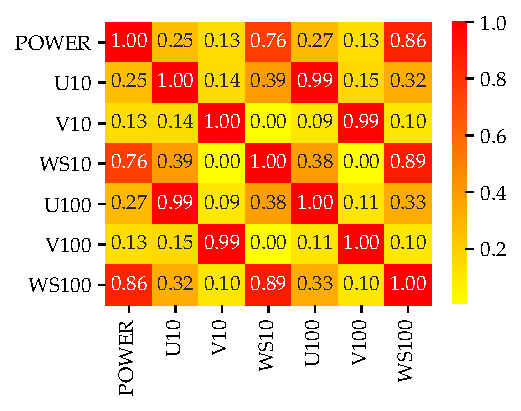
\includegraphics{figures/q1_corr_analysis.pdf}
  \caption{Correlation analysis of columns in \texttt{TrainData.csv}.}
  \label{fig:q1-corr-analysis}
\end{figure}

\begin{center}
  \csvautobooktabular{data/report_data/q1_RMSE.csv}
\end{center}

\begin{figure}
  \centering
  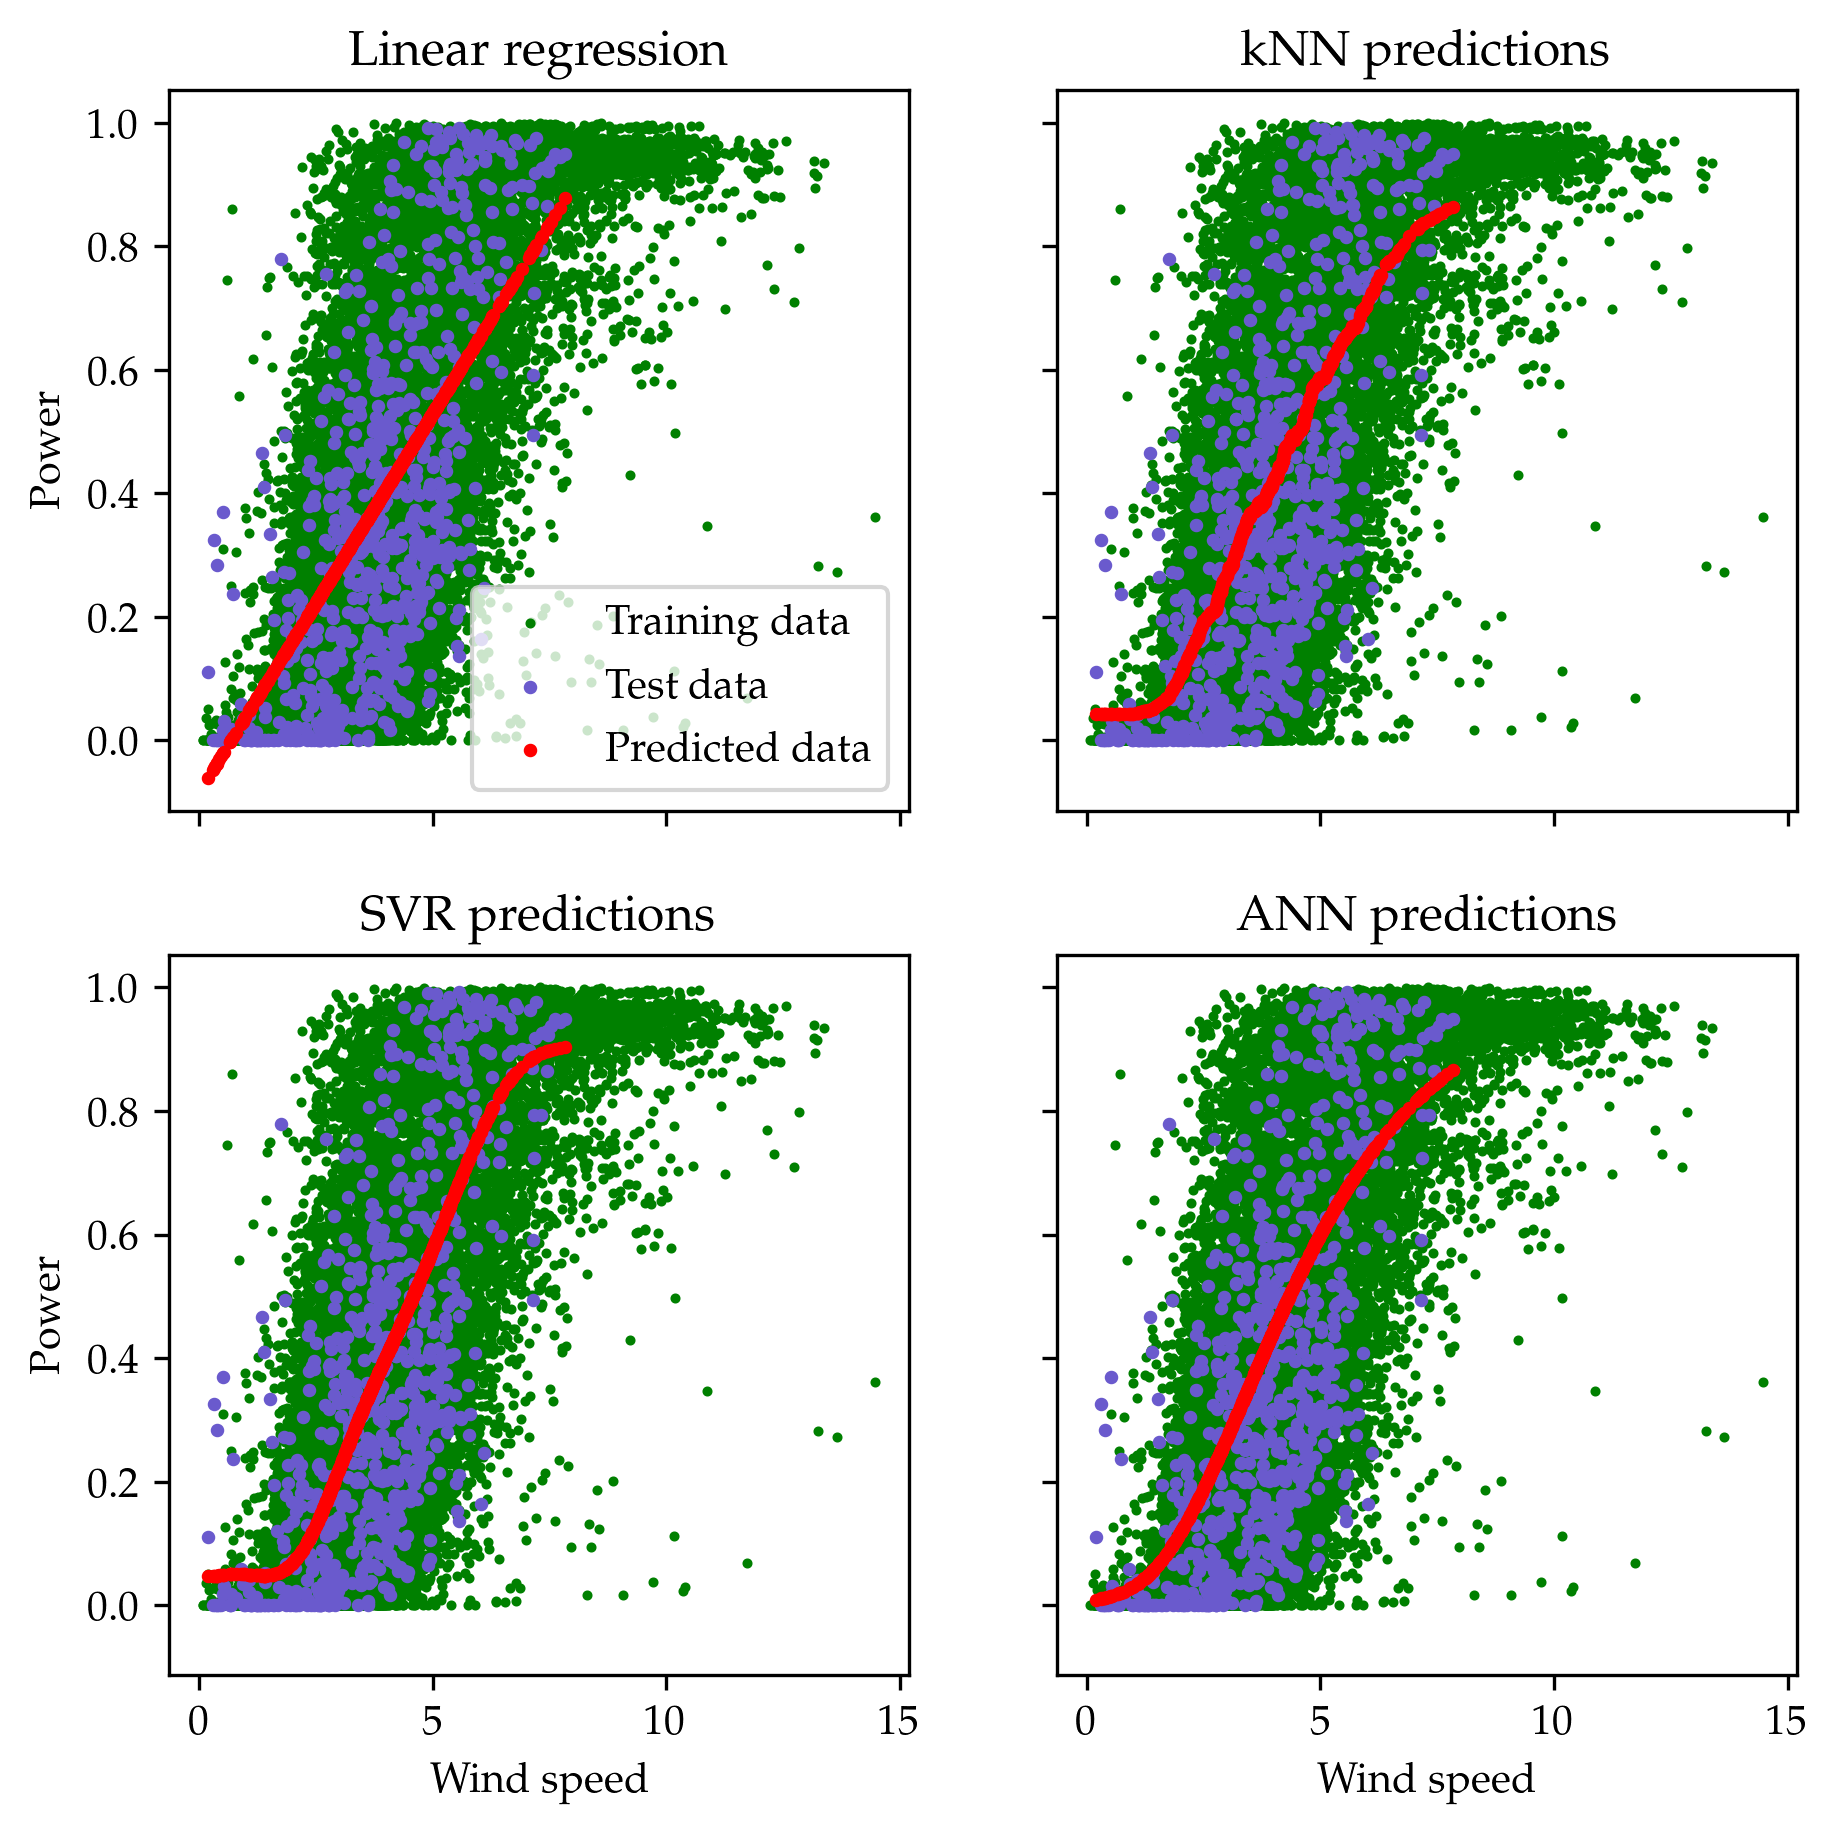
\includegraphics{figures/q1_prediction_plots.png}
  \caption{Plots of the various predictions for $f$ against the training and test data.}
  \label{fig:q1-prediction-plots}
\end{figure}

\begin{figure}
  \centering
  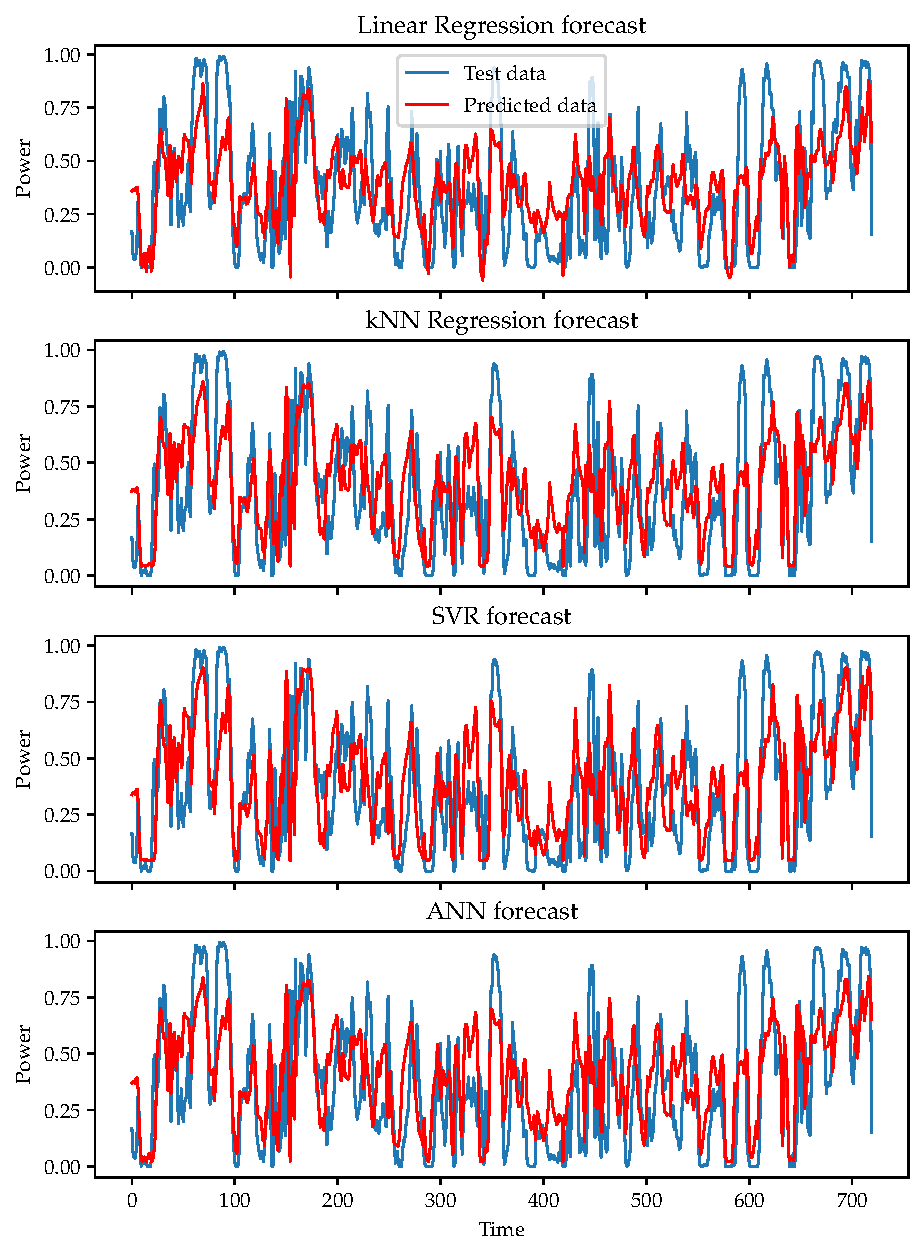
\includegraphics{figures/q1_forecast_plots}
  \caption{Plots of the forecast power output in November 2013 for different machine learning models.}
  \label{fig:q1-forecast-plots}
\end{figure}


\subsection*{Discussion}
In terms of RMSE, all the models perform similarly....

\subsubsection*{Accuracy of the results}
With all that said, consider the RMSEs of the four machine learning models on the training data:
\begin{center}
  \csvautobooktabular{data/report_data/q1_RMSE_training.csv}
\end{center}

As we can see, all the more advanced models outperform linear regression here...


\subsubsection*{Remark on neural network design complexity}
$f$ is a 1-dimensional function that seems very smooth on its domain.
Indeed, a quick test shows that a degree 3 polynomial fits the training data with a RMSE of \input{data/report_data/q1_RMSE_poly_training.txt}; about as good as any of the other models.
This shows that the power output function can be accurately described by only 4 real numbers.


\clearpage




\subsection*{Discussion}

Linear regression again was not......



\printbibliography


\end{document}


% Local Variables:
% TeX-engine: xetex
% End:
